\documentclass[11pt,openany]{article}

\usepackage{mathtools, commath}
% Packages for formatting
\usepackage[margin=1in]{geometry}
\usepackage{fancyhdr}
\usepackage{enumerate}
\usepackage{graphicx}
\usepackage{kotex}
\usepackage{arydshln} % Include this package
\usepackage{bbding}
\usepackage{amsmath}
\usepackage{amsthm}
\usepackage[dvipsnames,table]{xcolor}
\usepackage{amssymb, amsfonts}
\usepackage{wasysym}
\usepackage{footnote}
\usepackage{tablefootnote}
\usepackage{arydshln} % Include this package

% Fonts
\usepackage[T1]{fontenc}
\usepackage[utf8]{inputenc}
\usepackage{newpxtext,newpxmath}
\usepackage{sectsty}

% Define colors
\definecolor{TealBlue1}{HTML}{0077c2}
\definecolor{TealBlue2}{HTML}{00a5e6}
\definecolor{TealBlue3}{HTML}{b3e0ff}
\definecolor{TealBlue4}{HTML}{00293c}
\definecolor{TealBlue5}{HTML}{e6f7ff}

\definecolor{thmcolor}{RGB}{231, 76, 60}
\definecolor{defcolor}{RGB}{52, 152, 219}
\definecolor{lemcolor}{RGB}{155, 89, 182}
\definecolor{corcolor}{RGB}{46, 204, 113}
\definecolor{procolor}{RGB}{241, 196, 15}

\usepackage{color,soul}
\usepackage{soul}
\newcommand{\mathcolorbox}[2]{\colorbox{#1}{$\displaystyle #2$}}
\usepackage{cancel}
\newcommand\crossout[3][black]{\renewcommand\CancelColor{\color{#1}}\cancelto{#2}{#3}}
\newcommand\ncrossout[2][black]{\renewcommand\CancelColor{\color{#1}}\cancel{#2}}

\usepackage{hyperref}
\usepackage{booktabs}

% Chapter formatting
\definecolor{titleTealBlue}{RGB}{0,53,128}
\usepackage{titlesec}
\titleformat{\section}
{\normalfont\sffamily\Large\bfseries\color{titleTealBlue!100!gray}}{\thesection}{1em}{}
\titleformat{\subsection}
{\normalfont\sffamily\large\bfseries\color{titleTealBlue!50!gray}}{\thesubsection}{1em}{}

%Tcolorbox
\usepackage[most]{tcolorbox}
\usepackage{multirow}
\usepackage{multicol}
\usepackage{blindtext}

\usepackage[linesnumbered,ruled]{algorithm2e}
\usepackage{algpseudocode}
\usepackage{setspace}
\SetKwComment{Comment}{/* }{ */}
\SetKwProg{Fn}{Function}{:}{end}
\SetKw{End}{end}
\SetKw{DownTo}{downto}

% Define a new environment for algorithms without line numbers
\newenvironment{algorithm2}[1][]{
	% Save the current state of the algorithm counter
	\newcounter{tempCounter}
	\setcounter{tempCounter}{\value{algocf}}
	% redefine the algorithm numbering (remove prefix)
	\renewcommand{\thealgocf}{}
	\begin{algorithm}
	}{
	\end{algorithm}
	% Restore the algorithm counter state
	\setcounter{algocf}{\value{tempCounter}}
}

\usepackage{adjustbox}
% Header and footer formatting
\pagestyle{fancy}
\fancyhead{}
\fancyhf{}
\rhead{\textcolor{TealBlue2}{\large\textbf{리만의 복소해석을 토대로 얻는 내 수학적 시야 (2기)}}}%\rule{3cm}{0.4pt}}
\lhead{\textcolor{TealBlue2}{\large\textbf{수학의 즐거움, Enjoying Math}}}
% Define footer
%\newcommand{\footer}[1]{
%\begin{flushright}
%	\vspace{2em}
%	\includegraphics[width=2.5cm]{school_logo.jpg} \\
%	\vspace{1em}
%	\textcolor{TealBlue2}{\small\textbf{#1}}
%\end{flushright}
%}
%\rfoot{\large Department of Information Security, Cryptogrphy and Mathematics, Kookmin Uni.\includegraphics[height=1.5cm]{school_logo.jpg}}
\fancyfoot{}
\fancyfoot[C]{-\thepage-}

\usepackage{animate}
% Load the PDF and grab its total pages into \NumPages:
\newcount\NumPagesA
\pdfximage{riemann-tikz/secant_line_gif.pdf}% loads the PDF
\NumPagesA=\pdflastximagepages
\usepackage{tcolorbox}
\tcbset{colback=white, arc=5pt}

\definecolor{axiomcolor}{HTML}{a88bfa}
\definecolor{defcolor}{RGB}{52, 152, 219}
\definecolor{procolor}{RGB}{241, 196, 15}
\definecolor{thmcolor}{RGB}{231, 76, 60}
\definecolor{lemcolor}{RGB}{155, 89, 182}
\definecolor{corcolor}{RGB}{46, 204, 113}
\definecolor{execolor}{RGB}{90, 128, 127}

% Define a new command for the custom tcolorbox
\newcommand{\axiombox}[2][]{%
	\begin{tcolorbox}[colframe=axiomcolor, title={\color{white}\bfseries #1}]
		#2
	\end{tcolorbox}
}

\newcommand{\defbox}[2][]{%
	\begin{tcolorbox}[colframe=defcolor, title={\color{white}\bfseries #1}]
		#2
	\end{tcolorbox}
}

\newcommand{\lembox}[2][]{%
	\begin{tcolorbox}[colframe=lemcolor, title={\color{white}\bfseries #1}]
		#2
	\end{tcolorbox}
}

\newcommand{\probox}[2][]{%
	\begin{tcolorbox}[colframe=procolor, title={\color{white}\bfseries #1}]
		#2
	\end{tcolorbox}
}

\newcommand{\thmbox}[2][]{%
	\begin{tcolorbox}[colframe=thmcolor, title={\color{white}\bfseries #1}]
		#2
	\end{tcolorbox}
}

\newcommand{\corbox}[2][]{%
	\begin{tcolorbox}[colframe=corcolor, title={\color{white}\bfseries #1}]
		#2
	\end{tcolorbox}
}



\usepackage{amsthm}

% Define custom theorem styles
\newtheoremstyle{dotless} % Name of the style
{3pt} % Space above
{3pt} % Space below
{\itshape} % Body font
{} % Indent amount
{\bfseries} % Theorem head font
{} % Punctuation after theorem head
{2.5mm} % Space after theorem head
{} % Theorem head spec

\newtheoremstyle{definitionstyle} % Name of the style
{3pt} % Space above
{3pt} % Space below
{} % Body font
{} % Indent amount
{\bfseries} % Theorem head font
{.} % Punctuation after theorem head
{2.5mm} % Space after theorem head
{} % Theorem head spec

% Applying custom styles
\theoremstyle{dotless}
\newtheorem{theorem}{Theorem} % Theorem environment with section-wise numbering
\newtheorem{proposition}[theorem]{Proposition} % Theorem environment with section-wise numbering
\newtheorem{lemma}[theorem]{Lemma} % Lemma shares the counter with theorem
\newtheorem{corollary}[theorem]{Corollary} % Corollary shares the counter with theorem

\theoremstyle{definitionstyle}
\newtheorem*{observation}{\textcolor{Magenta}{Observation}}
\newtheorem{definition}{Definition} % Definition shares the counter with theorem
\newtheorem{example}{Example} % Example shares the counter with theorem
\newtheorem{exercise}{Exercise} % Example shares the counter with theorem
\newtheorem{remark}{Remark} % Remark shares the counter with theorem
\newtheorem*{note}{Note}

\newtheorem*{definition*}{Definition} % Definition shares the counter with theorem
\newtheorem*{example*}{Example} % Example shares the counter with theorem
\newtheorem*{exercise*}{\textcolor{violet}{Exercise}} % Example shares the counter with theorem
\newtheorem*{remark*}{Remark} % Remark shares the counter with theorem


\usepackage{tikz}
\usepackage{tikz-cd}
\usepackage{tikz-3dplot}
\usepackage{pgfplots}
\pgfplotsset{compat=newest} % Adjust to your version of pgfplots
\def\Circlearrowleft{\ensuremath{%
		\rotatebox[origin=c]{180}{$\circlearrowleft$}}}
\def\Circlearrowright{\ensuremath{%
		\rotatebox[origin=c]{180}{$\circlearrowright$}}}
\def\CircleArrowleft{\ensuremath{%
		\reflectbox{\rotatebox[origin=c]{180}{$\circlearrowleft$}}}}
\def\CircleArrowright{\ensuremath{%
		\reflectbox{\rotatebox[origin=c]{180}{$\circlearrowright$}}}}
\usetikzlibrary{
	3d, % For 3D drawing
	angles,
	arrows,
	arrows.meta,
	backgrounds,
	bending,
	calc,
	decorations.pathmorphing,
	decorations.pathreplacing,
	decorations.markings,
	fit,
	matrix,
	patterns,
	patterns.meta,
	positioning,
	quotes,
	shadows,
	shapes,
	shapes.geometric,
	tikzmark
}
\tikzset{
	% single mid‐path arrow
	mid arrow/.style={
		decoration={
			markings,
			mark=at position 0.5 with {\arrow{Stealth[scale=1.2]}}
		},
		postaction={decorate},
	},
	% style for field arrows
	field arrow/.style={
		-{Stealth[scale=1.0]},
		thick,
		blue!70!black,
	},
}
\newcommand{\ie}{\textnormal{i.e.}}
\newcommand{\rsa}{\mathsf{RSA}}
\newcommand{\rsacrt}{\mathsf{RSA}\textendash\mathsf{CRT}}
\newcommand{\inv}[1]{#1^{-1}}

%New Command
%\newcommand{\set}[1]{\left\{#1\right\}}
\newcommand{\N}{\mathbb{N}}
\newcommand{\Z}{\mathbb{Z}}
\newcommand{\Q}{\mathbb{Q}}
\newcommand{\R}{\mathbb{R}}
\newcommand{\cR}{\mathcal{R}}
\newcommand{\C}{\mathbb{C}}
\newcommand{\F}{\mathbb{F}}
\newcommand{\nbhd}{\mathcal{N}}
\newcommand{\Log}{\operatorname{Log}}
\newcommand{\Arg}{\operatorname{Arg}}
\newcommand{\pv}{\operatorname{P.V.}}

\newcommand{\of}[1]{\left( #1 \right)} 
%\newcommand{\abs}[1]{\left\lvert #1 \right\rvert}
%\newcommand{\norm}[1]{\left\| #1 \right\|}

\newcommand{\sol}{\textcolor{magenta}{\bf Sol}}
\newcommand{\conjugate}[1]{\overline{#1}}

\newcommand{\res}{\operatorname{res}}
\DeclareMathOperator*{\Res}{\operatorname{Res}}

%\renewcommand{\Re}{\operatorname{Re}}
%\renewcommand{\Im}{\operatorname{Im}}

\newcommand{\cyclic}[1]{\langle #1 \rangle}
\newcommand{\uniform}{\overset{\$}{\leftarrow}}
\newcommand{\xmark}{\textcolor{red}{\XSolidBrush}}
\newcommand{\vmark}{\textcolor{green!75!black}{\CheckmarkBold}}

\newcommand{\gen}[1]{\langle #1 \rangle}
\newcommand{\Gen}[1]{\left\langle #1 \right\rangle}

\newcommand{\img}[1]{\text{Img}(#1)}
\newcommand{\Img}[1]{\text{Img}\left(#1\right)}
\newcommand{\preimg}[1]{\text{Img}^{-1}(#1)}
\newcommand{\Preimg}[1]{\text{Img}^{-1}\left(#1\right)}

\newcommand{\relation}{\mathrel{\mathcal{R}}}
\newcommand{\injection}{\rightarrowtail}
\newcommand{\surjection}{\twoheadrightarrow}
\newcommand{\id}{\textnormal{id}}

\newcommand{\eqclass}[1]{\left[#1\right]}

% Define custom colors for O and X
\newcommand{\yes}{\textcolor{blue}{\bf \fullmoon}}
\newcommand{\no}{\textcolor{red}{\bf \texttimes}}

\DeclarePairedDelimiter\ceil{\lceil}{\rceil}
\DeclarePairedDelimiter\floor{\lfloor}{\rfloor}
%\renewcommand{\floor}[#1]{\lfloor #1\rfloor}
%\newcommand{\Floor}[#1]{\left\lfloor #1\right\rfloor}
%\newcommand{\ceil}[#1]{\lceil #1\rceil}
%\newcommand{\Ceil}[#1]{\left\lceil #1\right\rceil}

\newcommand{\topology}{\mathscr{T}}
\newcommand{\sequence}[1]{\langle #1\rangle}

% Topology
%\newcommand{\nbhd}{\mathcal{N}}

% Linear Algebra
\newcommand{\Span}{\operatorname{\normalfont span}}
\newcommand{\basis}{\mathcal{B}}
\newcommand{\card}[1]{\text{\normalfont card}(#1)}
\renewcommand{\vec}[1]{\mathbf{#1}}
\setstretch{1.25}

\begin{document}
\pagenumbering{arabic}
\begin{center}
	\huge\textbf{Riemann; Complex Analysis}\\
	\Large - HW1 -\\
	\vspace{0.5em}
	\large{Ji, Yong-hyeon}\\
%	\large{\ttfamily \url{https://github.com/Hacker-Code-J}}\\
	\vspace{0.5em}
	\normalsize{\today}\\
\end{center}

\noindent 
We cover the following topics in this note.
\begin{itemize}
	\item Vector Fields
	\item Line Integrals for Vector Fields
	\item Surface Integrals for Vector Fields
	\item TBA
\end{itemize}
\hrule\vspace{12pt}
\tableofcontents
%\newpage

\newpage
\section*{Scalar Function and Vector Fields}
\addcontentsline{toc}{section}{Scalar Function and Vector Fields}
A \textbf{scalar function} on \(\R^n\) is a real‑valued function of an \(n\)-tuple; that is,
\[
f:\R^n\to\R,\quad\vec{x}\mapsto f(\vec{x})=f(x_1,x_2,\dots,x_n).
%\fullfunction{f}{\R^n}{\R}{\vec{x}}{f(\vec{x})=f(x_1,x_2,\dots,x_n)}
\] where \(\vec{x}=(x_1,x_2,\dots,x_n)\in\R^n\) and\(f(\vec{x})\in\R\).
%
%et \(n=2\).  We exhibit two concrete \emph{scalar functions} on \(\R^2\setminus\{(0,0)\}\):
%
%\[
%\fullfunction{f_1}{\R^2\setminus\{(0,0)\}}{\R}{(x,y)}
%{f_1(x,y)\;=\;-\,\frac{y}{x^2+y^2}},
%\qquad
%\fullfunction{f_2}{\R^2\setminus\{(0,0)\}}{\R}{(x,y)}
%{f_2(x,y)\;=\;\frac{x}{x^2+y^2}}.
%\]
%
%Here \((x,y)\in\R^2\setminus\{(0,0)\}\) and \(f_i(x,y)\in\R\).  These functions assign to each point of the punctured plane a single real value, in accordance with the definition of a scalar function on \(\R^n\).
%
%
%\noindent\textbf{Polar‐coordinate form.}  Writing 
%\[
%x = r\cos\theta,\quad y = r\sin\theta,
%\quad r>0,\ \theta\in[0,2\pi),
%\]
%we obtain the equivalent descriptions in \((r,\theta)\)‐space:
%
%\[
%\fullfunction{f_1}{(0,\infty)\times[0,2\pi)}{\R}{(r,\theta)}
%{f_1(r,\theta) \;=\; -\,\frac{r\sin\theta}{r^2}
%	\;=\; -\,\frac{\sin\theta}{r}},
%\]
%
%\[
%\fullfunction{f_2}{(0,\infty)\times[0,2\pi)}{\R}{(r,\theta)}
%{f_2(r,\theta) \;=\; \frac{r\cos\theta}{r^2}
%	\;=\; \frac{\cos\theta}{r}}.
%\]
%
%In this form, the dependence on the angle \(\theta\) and the radial factor \(1/r\) is made explicit.
%
%
%\begin{center}
%\begin{tikzpicture}[scale=3,>=Stealth]
%	% Axes
%	\draw[->] (0,0) -- (1.2,0) node[right] {$x$};
%	\draw[->] (0,0) -- (0,1.2) node[above] {$y$};
%	
%	% Quarter‐circle with color ∝ x = cos(theta)
%	\foreach \t in {0,5,...,90} {
%		\pgfmathsetmacro{\tstart}{\t}
%		\pgfmathsetmacro{\tend}{min(\t+5,90)}            % don’t go past 90°
%		\pgfmathsetmacro{\mid}{(\tstart+\tend)/2}
%		% clamp to [0,1]
%		\pgfmathsetmacro{\col}{max(0,cos(\mid))}        
%		\draw[line width=1pt, red!\col!black]
%		({cos(\tstart)},{sin(\tstart)}) 
%		arc(\tstart:\tend:1);
%	}
%	
%	% orientation arrow
%	\draw[->, red!80!black, very thick]
%	(1,0) arc(0:15:1);
%	
%	% labels
%	\node[below right] at (1,0) {$C_1$};
%	\node[above right] at (0.6,0.6) 
%	{$\displaystyle\int_{C_1} x\,ds$};
%\end{tikzpicture}
%\begin{tikzpicture}[scale=3,>=Stealth]
%	% Axes
%	\draw[->] (0,0) -- (1.2,0) node[right] {$x$};
%	\draw[->] (0,0) -- (0,1.2) node[above] {$y$};
%	
%	% Full circle, constant density
%	\draw[blue!70!black, thick] (0,0) circle (1);
%	
%	% Tangent arrows at regular points
%	\foreach \ang in {0,45,...,315} {
%		\pgfmathsetmacro{\x}{cos(\ang)}
%		\pgfmathsetmacro{\y}{sin(\ang)}
%		% on r=1, F = (−y, x) but for ds we just show tangent dir
%		\draw[->, thick, blue!70!black]
%		(\x,\y) -- ++({-0.1*\y},{0.1*\x});
%	}
%	
%	% labels
%	\node[below right] at (1,0) {$C_2$};
%	\node[above right] at (0.6,0.6) 
%	{$\displaystyle\int_{C_2} (x^2+y^2)\,ds =2\pi$};
%\end{tikzpicture}
%\end{center}
%\begin{tikzpicture}[>=Stealth, thick, every label/.style={font=\small}]
%	
%	%% Domain: R^2 with unit circle
%	\begin{scope}
%		\draw[->] (-1.8,0) -- (1.8,0) node[right] {$x$};
%		\draw[->] (0,-1.8) -- (0,1.8) node[above] {$y$};
%		\draw (0,0) circle (1);
%		\node at (0,-2.1) {$\displaystyle \mathbb{R}^2$};
%		
%		% Sample points on circle
%		\coordinate (P1) at ({cos(60)},{sin(60)});
%		\fill (P1) circle (1.5pt);
%		\node[above left] at (P1) 
%		{$P_1\!\bigl(\tfrac12,\tfrac{\sqrt3}2\bigr)$};
%		
%		\coordinate (P2) at ({cos(30)},{sin(30)});
%		\fill (P2) circle (1.5pt);
%		\node[below right] at (P2) 
%		{$P_2\!\bigl(\tfrac{\sqrt3}2,\tfrac12\bigr)$};
%	\end{scope}
%	
%	%% Codomain: R^1 vertical line
%	\begin{scope}[xshift=6cm]
%		\draw[->] (0,-1.8) -- (0,1.8) node[above] {$z$};
%		\foreach \v in {-1,-0.5,0.5,1} {
%			\draw (-0.1,\v) -- (0.1,\v) node[right] {\(\v\)};
%		}
%		\node at (0,-2.1) {$\displaystyle \mathbb{R}^1$};
%	\end{scope}
%	
%	%% Mapping arrows
%	% f1 at theta=60: z = -sin(60) = -√3/2 ≈ -0.866
%	\draw[->, blue!70!black, bend left=20] 
%	(P1) to node[above, sloped] 
%	{\(\displaystyle f_1(P_1)=-\frac{y}{x^2+y^2}=-\tfrac{\sqrt3}{2}\)} 
%	(5.0,-0.866);
%	
%	% f2 at theta=30: z = cos(30) = √3/2 ≈ 0.866
%	\draw[->, red!70!black, bend right=20]
%	(P2) to node[below, sloped]
%	{\(\displaystyle f_2(P_2)=\frac{x}{x^2+y^2}=\tfrac{\sqrt3}{2}\)}
%	(5.0,0.866);
%	
%\end{tikzpicture}
%\begin{center}
	
%\begin{tikzpicture}[
%	>=Stealth,
%	every label/.style={font=\small},
%	thick
%	]
%	
%	%--- Domain: \mathbb{R}^2 plane ---
%	\begin{scope}
%		% axes
%		\draw[->] (-3,0) -- (3,0) node[right] {$x$};
%		\draw[->] (0,-3) -- (0,3) node[above] {$y$};
%		% domain label
%		\node at (0,-3.5) {$\displaystyle \mathbb{R}^2$};
%	\end{scope}
%	
%	%--- Codomain: \mathbb{R}^1 vertical line ---
%	\begin{scope}[xshift=8cm]
%		% vertical axis
%		\draw[->] (0,-3) -- (0,3) node[above] {$z$};
%		% ticks
%		\foreach \v in {-2,-1,1,2} {
%			\draw (-0.1,\v) -- (0.1,\v) node[right] {\(\v\)};
%		}
%		% codomain label
%		\node at (0,-3.5) {$\displaystyle \mathbb{R}^1$};
%	\end{scope}
%	
%	%--- Mapping arrows with formulas ---
%	\draw[->] (1.2,2.0) to[out=20,in=160]
%	node[above,midway] {\(\displaystyle f_1(x,y)=-\frac{y}{x^2+y^2}\)} (8,1.5);
%	
%	\draw[->] (-1.2,-2.0) to[out=-20,in=-160]
%	node[below,midway] {\(\displaystyle f_2(x,y)=\frac{x}{x^2+y^2}\)} (8,-1.5);
%	
%\end{tikzpicture}
	
\begin{center}
\begin{minipage}{.49\textwidth}\centering
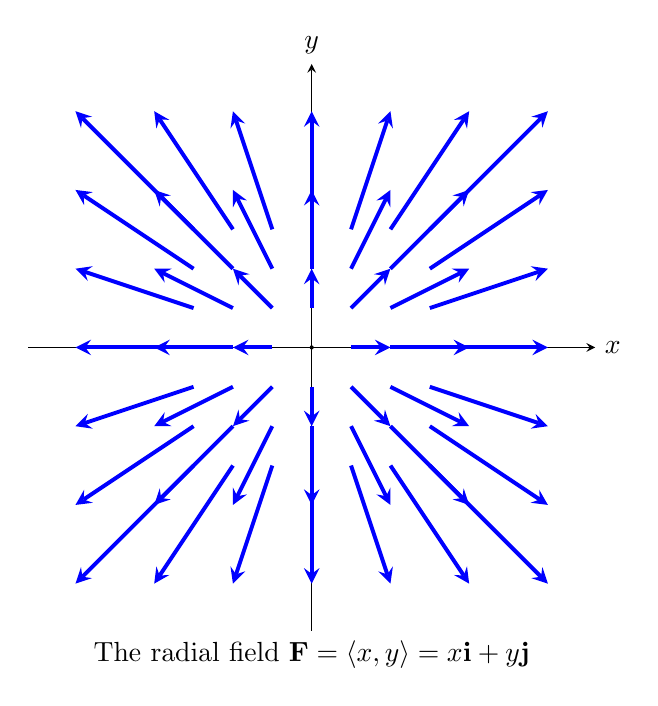
\begin{tikzpicture}[>=stealth, scale=.5]
%	\draw[dashed, gray!20] (-4,-4) grid (4,4);
% Draw coordinate axes
\draw[->] (-7.2,0) -- (7.2,0) node[right] {$x$};
\draw[->] (0,-7.2) -- (0,7.2) node[above] {$y$};
% Scaling factor for arrow lengths
\def\scale{1}
% Loop over integer grid points
\foreach \X in {-3,-2,-1,0,1,2,3} {
	\foreach \Y in {-3,-2,-1,0,1,2,3} {
		% Vector field components F = (vx, vy)
		\pgfmathsetmacro{\vx}{\X}
		\pgfmathsetmacro{\vy}{\Y}
		
		% Scaled arrow components (so arrows don't overlap too much)
		\pgfmathsetmacro{\ux}{\scale*\vx}
		\pgfmathsetmacro{\uy}{\scale*\vy}
		
		% Handle the singularity at (0,0)
		\ifnum\X=0
		\ifnum\Y=0
		% Zero vector as a dot
		\fill (0,0) circle (1.5pt);
		\else
		% Non‑zero vector: draw arrow
		\draw[->, line width=.5mm, blue]
		(\X,\Y) -- ++(\ux,\uy);
		\fi
		\else
		\draw[->, line width=.5mm, blue]
		(\X,\Y) -- ++(\ux,\uy);
		\fi
	}
}
\node[] at (0,-7.8) {The radial field $\textbf{F}=\gen{x,y}=x\textbf{i}+y\textbf{j}$};
\end{tikzpicture}
\end{minipage}\hfill
\begin{minipage}{.49\textwidth}\centering
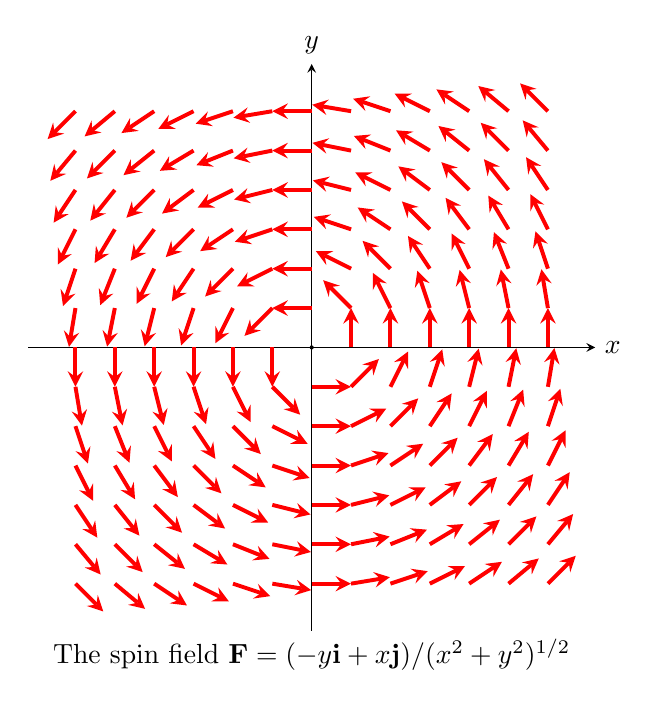
\begin{tikzpicture}[>=stealth, scale=.5]
%	\draw[dashed, gray!20] (-4,-4) grid (4,4);
% Axes
\draw[->] (-7.2,0) -- (7.2,0) node[right] {$x$};
\draw[->] (0,-7.2) -- (0,7.2) node[above] {$y$};
% Desired arrow length
\def\arrowlen{1}	
% Loop over integer grid points
\foreach \X in {-6,...,-2,-1,0,1,2,...,6} {
	\foreach \Y in {-6,...,-2,-1,0,1,2,...,6} {
		% Compute radius r = sqrt(x^2+y^2)
		\pgfmathsetmacro{\r}{sqrt(\X*\X + \Y*\Y)}
		
		\ifdim \r pt=0pt
		% At (0,0): singularity
		\fill (0,0) circle (1.5pt);
		\else
		% Compute unit‐tangent components then scale
		\pgfmathsetmacro{\dx}{(-\Y/\r)*\arrowlen}
		\pgfmathsetmacro{\dy}{(\X/\r)*\arrowlen}
		
		% Draw the arrow
		\draw[->, line width=.5mm, red]
		(\X,\Y) -- ++(\dx,\dy);
		\fi
	}
}
\node[] at (0,-7.8) {The spin field $\textbf{F}=(-y\textbf{i}+x\textbf{j})/(x^2+y^2)^{1/2}$};
\end{tikzpicture}
\end{minipage}
\end{center}
A \textbf{vector field} on \(\R^n\) is a function \[
\vec{F}:\R^n\to\R^n,\quad \vec{x}\mapsto\vec{F}(\vec{x})=(F_1(\vec{x}),F_2(\vec{x}),\dots,F_n(\vec{x})),
%\fullfunction{\vec{F}}{\R^n}{\R^n}{\vec{x}}{\vec{F}(\vec{x})	=\bigl(F_1(\vec{x}),\,F_2(\vec{x}),\,\dots,\,F_n(\vec{x})\bigr)},
\] where each component \(F_i:\R^n\to\R\) is itself a scalar function.

\newpage
\section*{Line Integrals}
\addcontentsline{toc}{section}{Line Integrals}
\subsection*{Line Integral of Scalar Function over Arc Length}
\addcontentsline{toc}{subsection}{Line Integral of Scalar Function over Arc Length}

\paragraph{Secant Lines \&  Tangent as a Limit}
\begin{center}
	\animateinline[autoplay,loop]{4}% 5 fps
	\multiframe{\the\NumPagesA}{i=1+1}{%
		\includegraphics[page=\i,width=\linewidth]{../riemann-tikz/secant_line_gif.pdf}%
	}
	\endanimateinline
\end{center}
For a curve $\gamma\colon t\mapsto\bigl(x(t),y(t)\bigr)$, the \emph{secant vector} over $[t,t+\Delta t]$ is
\[
\frac{\gamma(t+\Delta t)-\gamma(t)}{\Delta t}
= \Bigl(\tfrac{x(t+\Delta t)-x(t)}{\Delta t},\;\tfrac{y(t+\Delta t)-y(t)}{\Delta t}\Bigr).
\]
As $\Delta t \to 0$, these secants converge (if $\gamma$ is smooth) to
\[
\frac{d}{dt}\gamma(t)=\gamma'(t)
= \lim_{\Delta t\to0}
\frac{\gamma(t+\Delta t)-\gamma(t)}{\Delta t},
\]
which gives the \emph{tangent vector} at $\gamma(t)$.

\begin{center}
\begin{tikzpicture}[scale=7]
%	% Axes
%	\draw[->] (0,0) -- (1.2,0) node[right] {$x$};
%	\draw[->] (0,0) -- (0,1.2) node[above] {$y$};
%	
%	% Quarter circle C
%	\draw[blue!70!black,thick]
%	plot[samples=100,domain=0:90,smooth] (\x:1);
%	\node[blue!70!black,above right] at (45:1) {$C$};
%	
%	% Generic point P at t0
%	\def\t{40}  % degrees
%	\coordinate (P) at (\t:1);
%	\fill[red!80!black] (P) circle (0.8pt) node[above right] {$P=(\cos t,\sin t)$};
%	
%	% Radius OP
%	\draw[dashed] (0,0) -- (P) node[midway,left=2pt] {$1$};
%	
%	% Tangent vector r'(t)
%	\draw[->,very thick,orange!80!black]
%	(P) -- ++({\t+90}:0.25) 
%	node[right] {$\mathbf r'(t)$};
%	
%	% Small angle dt
%	\draw[->,purple!80!black,thick]
%	(0.7,0) arc(0:\t:0.7);
%	\node[purple!80!black] at ({\t/2}:0.8) {$\Delta t$};
	
	% axes
	\draw[->] (-.2,0) -- (1.5,0) node[below] {$x$};
	\draw[->] (0,-.2) -- (0,1.5) node[left]  {$y$};
	% unit circle
%	\draw[thick] (0,0) circle (1);%	
	\draw[thick] 
	plot[samples=100,domain=0:90,smooth] (\x:1);
	node[above right] at (45:1);
	
	% parameters
	\def\t{45}      % t0 in degrees
	\def\dt{10}     % delta t in degrees
	
	% points on the circle
	\coordinate (P)       at ({cos(\t)},{sin(\t)});
	\coordinate (Pminus)  at ({cos(\t-\dt)},{sin(\t-\dt)});
	\coordinate (Pplus)   at ({cos(\t+\dt)},{sin(\t+\dt)});
	
	% draw secant
	\draw[blue,thick,opacity=0.6]
	(Pminus) -- (Pplus)
	node[midway,above,sloped] {secant $\tfrac{\gamma(t_0+\Delta t)-\gamma(t_0-\Delta t)}{2\Delta t}$};
	
	% draw the point gamma(t0)
	\fill (P) circle (0.015) node[above right] {$\gamma(t_0)$};
	
	% tangent vector at t0
	% gamma'(t) = (-sin t, cos t)
	\coordinate (T) at ({-sin(\t)},{cos(\t)});
	\draw[red,->,very thick] (P) -- ++(T)
	node[right] {$\displaystyle\gamma'(t_0)=(-\sin t_0,\cos t_0)$};
	
%	% annotation of angles
%	\draw[gray,->] (0.3,0) arc (0:\t:0.3) node[midway,right] {$t_0$};
%	\draw[gray,->] (0.5,0) arc (0:{\t+\dt}:0.5) node[midway,above] {$t_0+\Delta t$};
%	\draw[gray,->] (0.7,0) arc (0:{\t-\dt}:0.7) node[midway,below] {$t_0-\Delta t$};
\end{tikzpicture}
\end{center}

\begin{frame}{Example: \(\frac{d}{dt}\) as a Linear Derivation}
	Let
	\[
	\gamma(t) = \bigl(x(t),\,y(t)\bigr)
	= \bigl(t^2,\;\sin t\bigr).
	\]
	Then the operator
	\[
	v_t \;=\;\left.\frac{d}{dt}\right|_{t}
	: C^\infty(\mathbb{R}^2)\;\longrightarrow\;\mathbb{R},
	\quad
	f \;\longmapsto\; \frac{d}{dt}\bigl(f(\gamma(t))\bigr)
	\]
	satisfies the Leibniz rule and in coordinates
	\[
	v_t
	= \sum_{i=1}^2 \dot x_i(t)\,\frac{\partial}{\partial x_i}
	= 2t\,\frac{\partial}{\partial x} \;+\;\cos t\,\frac{\partial}{\partial y}.
	\]
\end{frame}

\begin{frame}{Applying \(v_t\) to a Test Function}
	Take
	\[
	f(x,y) = x^2\,y.
	\]
	Then
	\[
	v_t(f)
	= 2t\,\frac{\partial}{\partial x}(x^2y)
	+ \cos t\,\frac{\partial}{\partial y}(x^2y)
	= 2t\,(2xy) + \cos t\,(x^2)
	\bigg|_{(x,y)=(t^2,\sin t)}
	= 4t^3\sin t \;+\; t^4\cos t.
	\]
	Equivalently,
	\[
	\frac{d}{dt}\bigl[f(\gamma(t))\bigr]
	= \frac{d}{dt}\bigl(t^4\sin t\bigr)
	= 4t^3\sin t + t^4\cos t.
	\]
\end{frame}

\begin{frame}{Verifying the Leibniz Property}
	For \(f(x,y)=x\), \(g(x,y)=y\):
	\[
	v_t(fg)
	= \frac{d}{dt}\bigl(x(t)\,y(t)\bigr)
	= \frac{d}{dt}\bigl(t^2\sin t\bigr)
	= 2t\sin t + t^2\cos t,
	\]
	while
	\[
	v_t(f)\,g + f\,v_t(g)
	= \bigl(2t\bigr)\bigl(\sin t\bigr)
	+ \bigl(t^2\bigr)\bigl(\cos t\bigr)
	= 2t\sin t + t^2\cos t.
	\]
	Hence \(v_t(fg)=v_t(f)\,g+f\,v_t(g)\).
\end{frame}
\[
\left.\frac{d}{dt}\right|_{t}\;:\;C^\infty(\mathbb{R}^n)\;\longrightarrow\;\mathbb{R},
\qquad
f\;\longmapsto\;
\frac{d}{dt}\bigl(f(\gamma(t))\bigr)
\;=\;
\sum_{i=1}^n \frac{dx_i}{dt}(t)\,\frac{\partial f}{\partial x_i}\bigl(\gamma(t)\bigr).
\]

\[
\frac{d}{dt}
\;=\;
\sum_{i=1}^n \frac{dx_i}{dt}(t)\,\frac{\partial}{\partial x_i}
\quad\text{so that}\quad
\frac{d}{dt}(f)
=\Bigl(\sum_i \dot x_i\,\partial_{x_i}\Bigr)[f].
\]

\begin{frame}{Secant Lines \& the Limit}
	\begin{itemize}
		\item For a curve $\gamma\colon t\mapsto\bigl(x(t),y(t)\bigr)$, the \emph{secant vector} over $[t,t+\Delta t]$ is
		\[
		\frac{\gamma(t+\Delta t)-\gamma(t)}{\Delta t}
		= \Bigl(\tfrac{x(t+\Delta t)-x(t)}{\Delta t},\;\tfrac{y(t+\Delta t)-y(t)}{\Delta t}\Bigr).
		\]
		\item As $\Delta t \to 0$, these secants converge (if $\gamma$ is smooth) to
		\[
		\frac{d}{dt}\gamma(t)=\gamma'(t)
		= \lim_{\Delta t\to0}
		\frac{\gamma(t+\Delta t)-\gamma(t)}{\Delta t},
		\]
		which gives the \emph{tangent vector} at $\gamma(t)$.
	\end{itemize}
\end{frame}

\section{Best Linear Approximation}
\begin{frame}{Derivative as Best Linear Approximation}
	\begin{itemize}
		\item The derivative is the unique linear map $D\gamma_t$ satisfying
		\[
		\gamma(t+\Delta t)
		= \gamma(t)
		+ D\gamma_t\bigl(\Delta t\bigr)
		+ o(\Delta t).
		\]
		\item In one–dimensional parameter space, $D\gamma_t(\Delta t)=\gamma'(t)\,\Delta t$.
		\item Thus $\gamma'(t)$ is the \emph{linear part} of the local approximation.
	\end{itemize}
\end{frame}

\section{Velocity Interpretation}
\begin{frame}{Velocity Vector Interpretation}
	\begin{itemize}
		\item View $\gamma(t)$ as the position of a particle at time $t$.
		\item Then
		\[
		\gamma'(t)
		= \frac{d}{dt}\gamma(t)
		\quad\text{is exactly the particle's velocity vector.}
		\]
		\item Velocity lies in the tangent space of the curve and measures \emph{instantaneous} speed \& direction.
	\end{itemize}
\end{frame}

\section{Differential–Geometric View}
\begin{frame}{Differential–Geometric View}
	\begin{itemize}
		\item A smooth curve is a map $\gamma\colon I\to M$.
		\item The tangent vector is the push‐forward
		\[
		\mathrm{d}\gamma_t\bigl(\tfrac{\partial}{\partial t}\bigr)
		\;\in\;T_{\gamma(t)}M.
		\]
		\item In coordinates $x^i$, one has
		\[
		\gamma'(t)
		= x^i{}'(t)\,\frac{\partial}{\partial x^i}.
		\]
	\end{itemize}
\end{frame}

\section{Summary}
\begin{frame}{Summary}
	\begin{itemize}
		\item Tangent vectors are the \emph{limit of secant vectors} as the interval shrinks.
		\item They arise as the \emph{best linear approximation} to the curve.
		\item Physically, they correspond to a particle's \emph{velocity}.
		\item In differential geometry, they are the \emph{push‐forward} of $\partial/\partial t$.
	\end{itemize}
\end{frame}

Let 
\[
\mathbf r\colon [a,b]\to\mathbb R^m,\quad
\mathbf r(t)=(x_1(t),\dots,x_m(t))
\]
be a $C^1$ parametrized curve.  We give two equivalent definitions of its length.

\bigskip

\noindent\textbf{1.\ Polygonal Approximation.}  Take a partition 
\(
a=t_0<t_1<\cdots<t_n=b
\),
and set
\[
\Delta S_k
=\bigl\|\mathbf r(t_k)-\mathbf r(t_{k-1})\bigr\|
=\sqrt{\sum_{i=1}^m\bigl[x_i(t_k)-x_i(t_{k-1})\bigr]^2}\,.
\]
Then
\[
L(C)
=\lim_{\max|t_k-t_{k-1}|\to0}
\sum_{k=1}^n\Delta S_k
\;=\;
\lim_{n\to\infty}\sum_{k=1}^n\Delta S_k.
\]
For example, if $m=2$ and 
\(\mathbf r(t)=(\cos t,\sin t)\), $t\in[0,\pi/2]$, one finds 
\(\Delta S_k\approx|t_k-t_{k-1}|\) and hence 
$L=\int_0^{\pi/2}1\,dt=\tfrac\pi2$.

\bigskip

\noindent\textbf{2.\ Differential‐Form Definition.}  In coordinates, let
\[
dx_i = x_i'(t)\,dt,
\quad
i=1,\dots,m.
\]
Define the line‐element (a $1$‐form)
\[
ds
=\sqrt{(dx_1)^2+(dx_2)^2+\cdots+(dx_m)^2}
=\sqrt{\sum_{i=1}^m (dx_i)^2}\,.
\]
Then the arc‐length is
\[
L(C)
=\int_C ds
=\int_a^b \sqrt{\sum_{i=1}^m \bigl(x_i'(t)\bigr)^2}\;dt
=\int_a^b \bigl\|\mathbf r'(t)\bigr\|\,dt.
\]
In particular:
\begin{itemize}
	\item \emph{2-D:} $ds=\sqrt{dx^2+dy^2}$, so 
	$L=\int_C\sqrt{dx^2+dy^2}$.  
	
	\item \emph{3-D:} $ds=\sqrt{dx^2+dy^2+dz^2}$, so 
	$L=\int_C\sqrt{dx^2+dy^2+dz^2}$.
	
	\item \emph{$n$-D:} $ds=\sqrt{\sum_{i=1}^n dx_i^2}$, so 
	$L=\int_Cds$ as above.
\end{itemize}

\bigskip

\noindent\textbf{Example (Quarter‐Circle).}  On $C\!:x^2+y^2=1$, 
$\mathbf r(t)=(\cos t,\sin t)$, $t\in[0,\pi/2]$, we have
\[
ds
=\sqrt{(-\sin t)^2+(\cos t)^2}\,dt
=\;1\cdot dt,
\]
so
\[
L
=\int_0^{\pi/2}ds
=\int_0^{\pi/2}1\,dt
=\frac\pi2.
\]
\newpage
On \(\R^n\) let \((x^1,\dots,x^n)\) be Cartesian coordinates.  Define the \emph{line element} (a differential 1-form)
\[
\boxed{
	ds \;=\;\sqrt{(dx^1)^2+(dx^2)^2+\cdots+(dx^n)^2}
	\;=\;\sqrt{\sum_{i=1}^n(dx^i)^2}\,.
}
\]
Then for any smooth curve
\[
\mathbf r\colon [a,b]\longrightarrow\R^n,
\quad
t\mapsto \bigl(x^1(t),\dots,x^n(t)\bigr),
\]
its \emph{arc‐length} is the pullback of \(ds\) integrated over \([a,b]\):
\[
\boxed{
	L(C)
	\;=\;
	\int_C ds
	\;=\;
	\int_a^b \bigl\|\,\mathbf r'(t)\bigr\|\,dt
	\;=\;
	\int_a^b \sqrt{\sum_{i=1}^n \bigl(x^i{}'(t)\bigr)^2}\;dt.
}
\]
In particular:
\begin{itemize}
	\item \emph{2-D:} \(ds=\sqrt{dx^2+dy^2}\), so 
	\(\displaystyle L=\int_C\sqrt{dx^2+dy^2}\).
	\item \emph{3-D:} \(ds=\sqrt{dx^2+dy^2+dz^2}\), so 
	\(\displaystyle L=\int_C\sqrt{dx^2+dy^2+dz^2}\).
	\item \emph{\(n\)-D:} as above with \(n\) differentials.
\end{itemize}

\bigskip

\noindent\textbf{Justification.}  By definition of the pullback,
\[
\mathbf r^*(dx^i)=x^i{}'(t)\,dt,
\]
so
\[
\mathbf r^*(ds)
=\sqrt{\sum_i\bigl(x^i{}'(t)\,dt\bigr)^2}
=\sqrt{\sum_i\bigl(x^i{}'(t)\bigr)^2}\;dt
=\|\mathbf r'(t)\|\,dt.
\]

\noindent Hence 
\(\displaystyle L=\int_C ds=\int_a^b\|\mathbf r'(t)\|\,dt\), 
recovering the usual formula.  


\newpage

We begin with the intuitive idea: approximate a smooth curve by joining successive points with straight chords, sum their lengths, and let the mesh of the partition tend to zero.  Concretely:

\bigskip

\subsection*{1. Planar Curves (2-D)}

Let \(C\) be a smooth curve in the plane parametrized by 
\[
\mathbf r(t)=(x(t),y(t)),\quad t\in[a,b],
\]
with \(x,y\in C^1\).  Choose a partition
\[
a=t_0<t_1<\cdots<t_n=b,
\]
and for each \(k\) let
\[
\Delta S_k
=\bigl\|\mathbf r(t_k)-\mathbf r(t_{k-1})\bigr\|
=\sqrt{\bigl[x(t_k)-x(t_{k-1})\bigr]^2
	+\bigl[y(t_k)-y(t_{k-1})\bigr]^2}\,.
\]
Then the length of \(C\) is
\[
L(C)
=\lim_{\max|t_k-t_{k-1}|\to0}
\sum_{k=1}^n\Delta S_k
=\lim_{n\to\infty}\sum_{k=1}^n\Delta S_k.
\]
\emph{Example.}  For the quarter‐circle of radius 1,
\(\mathbf r(t)=(\cos t,\sin t)\), \(t\in[0,\pi/2]\), one computes
\[
\Delta S_k
\approx\sqrt{2-2\cos(t_k-t_{k-1})}
\;\approx\;|t_k-t_{k-1}|
\quad(\text{for small }\Delta t),
\]
so summing and taking limits yields
\(\displaystyle L=\int_0^{\pi/2}1\,dt=\frac\pi2\).

\bigskip

\subsection*{2. Space Curves (3-D)}

Let \(C\) be a smooth curve in space,
\(\mathbf r(t)=(x(t),y(t),z(t))\), \(t\in[a,b]\).  With the same partition,
\[
\Delta S_k
=\sqrt{\bigl[x(t_k)-x(t_{k-1})\bigr]^2
	+\bigl[y(t_k)-y(t_{k-1})\bigr]^2
	+\bigl[z(t_k)-z(t_{k-1})\bigr]^2}\,,
\]
and 
\[
L(C)
=\lim_{n\to\infty}\sum_{k=1}^n\Delta S_k
=\int_a^b\sqrt{x'(t)^2+y'(t)^2+z'(t)^2}\,dt.
\]
\emph{Example.}  For the helix 
\(\mathbf r(t)=(\cos t,\sin t,t)\), \(t\in[0,2\pi]\), one finds
\(\|\mathbf r'(t)\|=\sqrt{\sin^2t+\cos^2t+1}=\sqrt2\),
so \(L=\int_0^{2\pi}\!\sqrt2\,dt=2\pi\sqrt2\).

\bigskip

\subsection*{3. Curves in \(\R^n\)}

In \(\R^n\), a smooth curve \(\mathbf r(t)=(x_1(t),\dots,x_n(t))\) admits
\[
\Delta S_k
=\sqrt{\sum_{i=1}^n\bigl[x_i(t_k)-x_i(t_{k-1})\bigr]^2},
\]
and
\[
L(C)
=\lim_{n\to\infty}\sum_{k=1}^n\Delta S_k
=\int_a^b\sqrt{\sum_{i=1}^n [x_i'(t)]^2}\,dt.
\]

\bigskip

\noindent\textbf{Why this works:} each chord  
\(\mathbf r(t_k)-\mathbf r(t_{k-1})\)  
approximates \(\mathbf r'(t)\,\Delta t\), so
\(\|\Delta\mathbf r\|\approx\|\mathbf r'(t)\|\Delta t\),  
and summing gives the Riemann integral of \(\|\mathbf r'(t)\|\).


Consider the quarter‐circle \[
C\colon x^2 + y^2 = 1,\quad x\ge0,\;y\ge0.
\]
A natural parametrization is
\[
\mathbf r\colon 
[0,\tfrac\pi2]\;\longrightarrow\;\mathbb{R}^2,
\qquad
\mathbf r(t) = \bigl(\cos t,\;\sin t\bigr).
\]
Then
\[
\mathbf r'(t)
= \bigl(-\sin t,\;\cos t\bigr),
\]
and its Euclidean norm is
\[
\bigl\|\mathbf r'(t)\bigr\|
= \sqrt{(-\sin t)^2 + (\cos t)^2}
=\sqrt{\sin^2t + \cos^2t}
=1.
\]
By the definition of arc length,
\[
\text{Length}(C)
= \int_{0}^{\pi/2} \bigl\|\mathbf r'(t)\bigr\|\,dt
= \int_{0}^{\pi/2}1\,dt
= \left[t\right]_{0}^{\pi/2}
= \frac\pi2.
\]
\[
\boxed{\;\text{Hence the quarter‐circle has length } \frac\pi2.\!}
\]
\qed


\begin{center}
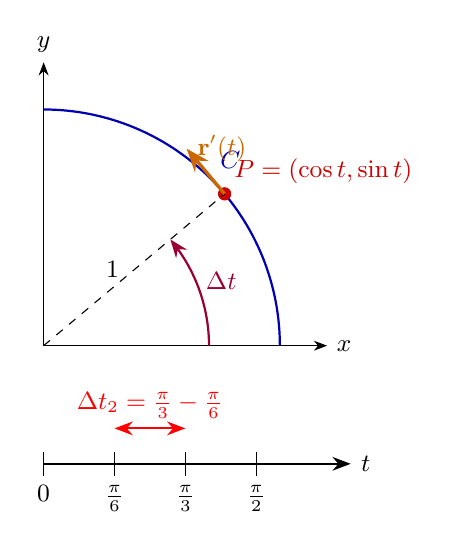
\begin{tikzpicture}[>=Stealth,scale=3,font=\small]
	% Axes
	\draw[->] (0,0) -- (1.2,0) node[right] {$x$};
	\draw[->] (0,0) -- (0,1.2) node[above] {$y$};
	
	% Quarter circle C
	\draw[blue!70!black,thick]
	plot[samples=100,domain=0:90,smooth] (\x:1);
	\node[blue!70!black,above right] at (45:1) {$C$};
	
	% Generic point P at t0
	\def\t{40}  % degrees
	\coordinate (P) at (\t:1);
	\fill[red!80!black] (P) circle (0.8pt) node[above right] {$P=(\cos t,\sin t)$};
	
	% Radius OP
	\draw[dashed] (0,0) -- (P) node[midway,left=2pt] {$1$};
	
	% Tangent vector r'(t)
	\draw[->,very thick,orange!80!black]
	(P) -- ++({\t+90}:0.25) 
	node[right] {$\mathbf r'(t)$};
	
	% Small angle dt
	\draw[->,purple!80!black,thick]
	(0.7,0) arc(0:\t:0.7);
	\node[purple!80!black] at ({\t/2}:0.8) {$\Delta t$};
	
	% Corresponding arc Δs
%	\draw[decorate,decoration={markings,mark=between positions 0.1 and 0.9 step 0.1 with {\arrow[scale=0.8]{>}}},red,thick]
%	({\t-2}:1) arc({\t-2}:{\t+2}:1);
%	\node[red] at ({\t}:1.1) {$\Delta s$};
%	
	% Relationship label
%	\node[align=center] at (0.5,-0.3) 
%	{On the unit circle,\\[-2pt]
%		\(\Delta s = 1\cdot \Delta t = \Delta t\).};
	
	\begin{scope}[yshift=-.5cm]
		\draw[->,thick] (0,0) -- (1.3,0) node[right] {$t$};
		\foreach \t/\lab in {
%			0/$0$, 0.5236/$\tfrac\pi6$, 1.0472/$\tfrac\pi3$, 1.5708/$\tfrac\pi2$
			0/$0$, .3/$\tfrac\pi6$, .6/$\tfrac\pi3$, .9/$\tfrac\pi2$
		}{
			\draw (\t,0.05)--(\t,-0.05) node[below] {\lab};
		}
		% Δt_2 between π/6 and π/3
		\draw[<->,thick,red] (0.3,0.15) -- node[above] {$\Delta t_2=\tfrac\pi3-\tfrac\pi6$} (.6,0.15);
	\end{scope}
\end{tikzpicture}
\end{center}
Let $I=[a,b]\subset\mathbb{R}$ and let 
\[
\mathbf r\colon I\;\longrightarrow\;\mathbb{R}^n,
\quad t\;\mapsto\;\mathbf r(t)
\]
be a continuously differentiable (\(C^1\)) curve.  

\begin{definition}[Arc Length]
	The \emph{arc length} of the curve $\mathbf r(t)$ over the interval $[a,b]$ is
	\[
	L[\mathbf r]
	\;=\;
	\sup_{\,\mathcal P}\;
	\sum_{i=1}^N
	\bigl\|\mathbf r(t_i)-\mathbf r(t_{i-1})\bigr\|,
	\]
	where the supremum is taken over all partitions 
	\(\mathcal P\colon a=t_0<t_1<\cdots<t_N=b\) of the interval $[a,b]$, and $\|\cdot\|$ is the Euclidean norm on~$\R^n$.
\end{definition}

\begin{remark}[Motivation]
	\ 
	\begin{itemize}
		\item We approximate the smooth curve by a polygonal path joining the points 
		\(\mathbf r(t_0),\mathbf r(t_1),\dots,\mathbf r(t_N)\).  
		\item Each segment has length $\|\mathbf r(t_i)-\mathbf r(t_{i-1})\|$.  
		\item Taking the supremum over all finer and finer partitions captures the intuitive “length of the curve.”  
		\item This definition reduces to the usual distance when $\mathbf r(t)$ is a straight line.
	\end{itemize}
\end{remark}

\begin{theorem}
	If $\mathbf r\in C^1([a,b],\R^n)$, then the above supremum equals the integral
	\[
	L[\mathbf r]
	\;=\;
	\int_a^b
	\bigl\|\mathbf r\,'(t)\bigr\|\;dt.
	\]
\end{theorem}

\begin{proof}[Sketch of proof]
	\ 
	\begin{enumerate}
		\item On each subinterval $[t_{i-1},t_i]$, the Mean Value Theorem gives
		\(\mathbf r(t_i)-\mathbf r(t_{i-1})
		=\mathbf r\,'(\xi_i)\,(t_i-t_{i-1})\) for some $\xi_i\).  
		\item Hence 
		\(\|\mathbf r(t_i)-\mathbf r(t_{i-1})\|
		=\|\mathbf r\,'(\xi_i)\|\,(t_i-t_{i-1})\).  
		\item Summing and passing to the limit as the mesh of the partition goes to zero yields the Riemann integral 
		\(\int_a^b\|\mathbf r\,'(t)\|\,dt\).  
	\end{enumerate}
\end{proof}

\bigskip

\noindent\textbf{Why this definition?}
\begin{itemize}
	\item It agrees with our geometric intuition of “length” via polygonal approximation.
	\item It is \emph{reparametrization invariant}: if one changes $t$–coordinate without reversing direction, the integral of $\|\mathbf r\,'(t)\|\,dt$ remains the same.
	\item It generalizes the classical arclength formula for graphs $y=y(x)$:
	\[
	L=\int_a^b\sqrt{1+(y'(x))^2}\,dx.
	\]
\end{itemize}


\begin{definition*}[Line Integral of Scalar Function over Arc Length]
	Let $f:\R^n\to\R$ be a scalar function, and let $C$ be a piecewise smooth curve in 
	$\R^n$ given by a smooth parameterization: \[
	\gamma:[a,b]\to\R^n,\quad t\mapsto \gamma(t)=(x_1(t),x_2(t),\dots,x_n(t)).
	\] Then the \emph{arc length} of the curve $C$ from $t=a$ to $t=b$ is defined by \[
	L(\gamma):=\int_a^b\norm{\frac{ d\gamma}{dt}}\; dt,\quad\text{where}\; \norm{\frac{d\gamma}{dt}}=\sqrt{\left(\frac{dx_1}{dt}\right)^2+\left(\frac{dx_1}{dt}\right)^2+\cdots + \left(\frac{dx_1}{dt}\right)^2}.
	\]The \textbf{line integral of the scalar function} $f$ along the curve $C$ with respect to arc length is defined by \[
	\int_C f\; ds :=\int_a^bf(\gamma(t))\norm[0]{\gamma'(t)}\; dt.
	\] Here, $ds=\norm[0]{\gamma'(t)}\; dt$ is the \emph{infinitesimal arc length}.
\end{definition*}


\subsection*{Line Integral of Vector Fields}
\addcontentsline{toc}{subsection}{Line Integral of Vector Fields}

Excellent — this is a key question for understanding how **vector calculus** connects with **differential forms** and notation. Let's walk through how to **rigorously deduce**:

\[
\int_C F_1\,dx + F_2\,dy
\quad \text{from} \quad
\int_C \vec{F} \cdot d\vec{r}
\]
for a vector field \( \vec{F}(x,y) = (F_1(x,y), F_2(x,y)) \).

---



 **Step 1: Parametrize the Curve \( C \)**

Let \( \gamma: [a, b] \to \mathbb{R}^2 \) be a smooth parameterization of the curve \( C \), given by:
\[
\gamma(t) = (x(t), y(t)), \quad t \in [a, b].
\]

Then the **derivative of the curve** is:
\[
\gamma'(t) = (x'(t), y'(t)),
\]
and the **differential displacement** is:
\[
d\vec{r} = \gamma'(t)\,dt = (dx, dy) = (x'(t)\,dt, y'(t)\,dt).
\]

---

 **Step 2: Write the Line Integral of \( \vec{F} \)**

The **vector line integral** is defined as:
\[
\int_C \vec{F} \cdot d\vec{r}
= \int_a^b \vec{F}(\gamma(t)) \cdot \gamma'(t)\,dt
= \int_a^b \left[ F_1(x(t), y(t))\,x'(t) + F_2(x(t), y(t))\,y'(t) \right] dt.
\]

---

 **Step 3: Recognize the Total Differentials**

From calculus, we know:
\[
dx = x'(t)\,dt, \quad dy = y'(t)\,dt.
\]

Substitute into the integral:
\[
\int_a^b F_1(x(t), y(t))\,dx + F_2(x(t), y(t))\,dy.
\]

So we have:
\[
\int_C \vec{F} \cdot d\vec{r}
= \int_a^b F_1(x(t), y(t))\,dx + F_2(x(t), y(t))\,dy
= \int_C F_1\,dx + F_2\,dy.
\]

---

Final Deduction

Thus:
\[
\boxed{
	\int_C \vec{F} \cdot d\vec{r}
	= \int_C F_1\,dx + F_2\,dy
}
\]
where:
- \( \vec{F} = (F_1, F_2) \),
- \( d\vec{r} = (dx, dy) \),
- The dot product \( \vec{F} \cdot d\vec{r} = F_1\,dx + F_2\,dy \).

---

 Interpretation

- The vector line integral becomes an integral of a **1-form**:  
\[
\vec{F} \cdot d\vec{r} \quad \leftrightarrow \quad F_1\,dx + F_2\,dy.
\]
- The dot product turns into a sum of **components times differentials**.

---

Would you like to go one step further and express this in terms of pullbacks or show how it generalizes to \( \mathbb{R}^3 \)?

\newpage
Let \(U\subseteq\mathbb{R}^n\) be an open set and 
\(\displaystyle\mathbf F:U\to\mathbb{R}^n\) a continuous vector field.  
Suppose \(C\subset U\) is a smooth curve parametrized by
\[
\mathbf r\colon [a,b]\;\longrightarrow\;\mathbb{R}^n,
\quad
t\;\mapsto\;\mathbf r(t),
\]
with nonzero velocity \(\mathbf r'(t)\).  Then the \emph{line integral} of \(\mathbf F\) along \(C\) is defined by
\[
\boxed{
	\int_C\mathbf F\!\cdot d\mathbf r
	\;=\;
	\int_a^b
	\mathbf F\bigl(\mathbf r(t)\bigr)\;\cdot\;\mathbf r'(t)\;dt
	\;=\;
	\int_a^b
	\sum_{i=1}^n F_i\bigl(\mathbf r(t)\bigr)\,x_i'(t)\;dt,
}
\]
where \(\mathbf r(t)=(x_1(t),\dots,x_n(t))\) and 
\(\mathbf F=(F_1,\dots,F_n)\).  

\medskip

\noindent
This integral “accumulates” at each infinitesimal step \(dt\) the projection of \(\mathbf F\) onto the tangent vector \(\mathbf r'(t)\), yielding a single real number that captures the \emph{circulation} or \emph{work} of \(\mathbf F\) along \(C\).

\bigskip

\noindent\textbf{Example.}  Take \(n=2\) and 
\(\displaystyle \mathbf F(x,y)
=\Bigl(-\tfrac{y}{x^2+y^2},\,\tfrac{x}{x^2+y^2}\Bigr)\)
on \(U=\mathbb{R}^2\setminus\{(0,0)\}\).  Let \(C\) be the unit circle 
\(\;x^2+y^2=1\), counterclockwise.  Parametrize
\(\mathbf r(t)=(\cos t,\sin t)\), \(t\in[0,2\pi]\).  Then
\[
\mathbf r'(t)=(-\sin t,\cos t),\qquad
\mathbf F\bigl(\mathbf r(t)\bigr)
=\bigl(-\sin t,\cos t\bigr),
\]
so
\[
\int_C\mathbf F\!\cdot d\mathbf r
=\int_0^{2\pi}
\bigl(-\sin t,\cos t\bigr)\cdot(-\sin t,\cos t)\;dt
=\int_0^{2\pi}
\bigl(\sin^2t+\cos^2t\bigr)\;dt
=2\pi.
\]
Thus the total circulation (or “work”) of \(\mathbf F\) around the unit circle is \(2\pi\).


\paragraph{{\color{magenta}Problem\;\#1} (Line Integral around Unit Circle).} Let \( C \subset \mathbb{R}^2 \) be the unit circle defined by \[
C: x^2 + y^2 = 1,
\] traversed in the \emph{counterclockwise direction}. Let the vector field \( \vec{F}: \mathbb{R}^2 \setminus \{(0,0)\} \to \mathbb{R}^2 \) be defined by \[
\vec{F}(x, y) = \left( \frac{-y}{x^2 + y^2},\; \frac{x}{x^2 + y^2} \right).
\] Evaluate the \emph{line integral} of \( \vec{F} \) along \( C \): \[
\oint_C \vec{F} \cdot d\vec{r}.
\]
\begin{proof}[\sol]
\ \begin{center}
\begin{minipage}{.49\textwidth}\centering
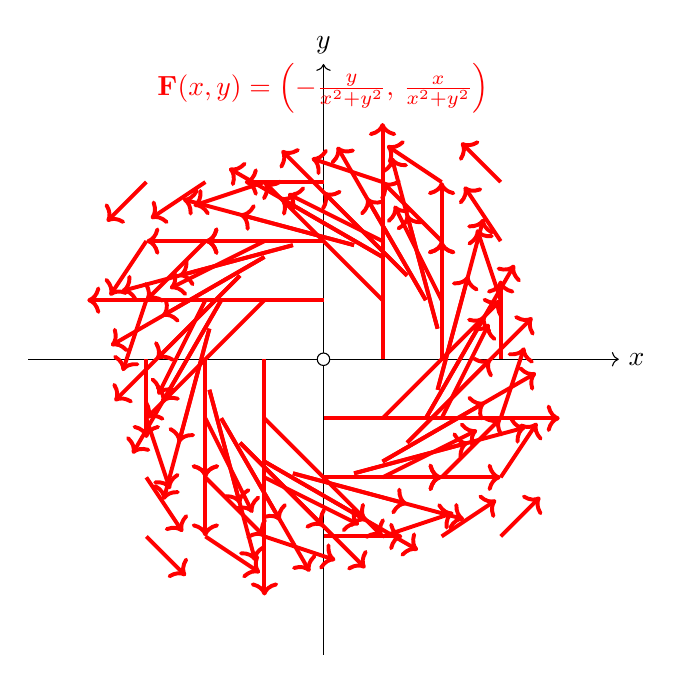
\begin{tikzpicture}[scale=1.5]
%	\draw[dashed, gray!20] (-4,-4) grid (4,4);
	% Axes
	\draw[->] (-2.5,0) -- (2.5,0) node[right] {$x$};
	\draw[->] (0,-2.5) -- (0,2.5) node[above] {$y$};
	% Desired arrow length
	\def\arrowlen{1}	
	% Loop over integer grid points
	\foreach \X in {-1.5,-1,-.5,0,.5,1,1.5} {
		\foreach \Y in {-1.5,-1,-.5,0,.5,1,1.5} {
			% Compute radius r = sqrt(x^2+y^2)
			\pgfmathsetmacro{\r}{\X*\X + \Y*\Y}
			
			\ifdim \r pt=0pt
			% At (0,0): singularity
			\fill[white,draw=black] (0,0) circle (1.5pt);
			\else
			% Compute unit‐tangent components then scale
			\pgfmathsetmacro{\dx}{(-\Y/\r)*\arrowlen}
			\pgfmathsetmacro{\dy}{(\X/\r)*\arrowlen}
			
			% Draw the arrow
			\draw[->, line width=.5mm, red]
			(\X,\Y) -- ++(\dx,\dy);
			\fi
		}
	}
	\foreach \t in {0,15,...,345}{
		\pgfmathsetmacro\x{cos(\t)}
		\pgfmathsetmacro\y{sin(\t)}
		% On r=1, F = (-y,x)
		\pgfmathsetmacro\dx{(-\y)*\arrowlen}
		\pgfmathsetmacro\dy{(\x)*\arrowlen}
		\draw[->, line width=.5mm, red] 
		(\x,\y) -- ++(\dx,\dy);
	}
	\def\arrowlen{1.5}
	\foreach \t in {0,15,...,345}{
		\pgfmathsetmacro\x{cos(\t)}
		\pgfmathsetmacro\y{sin(\t)}
		% On r=1, F = (-y,x)
		\pgfmathsetmacro\dx{(-\y)*\arrowlen}
		\pgfmathsetmacro\dy{(\x)*\arrowlen}
		\draw[->, line width=.5mm, red] 
		(\x,\y) -- ++(\dx,\dy);
	}
	
	%--- Annotations -----------------------------------------
	\node[above, red] at (0,2)
	{$\vec{F}(x,y)=\left(-\tfrac{y}{x^2+y^2},\,\tfrac{x}{x^2+y^2}\right)$};
\end{tikzpicture}
\end{minipage}
\begin{minipage}{.49\textwidth}\centering
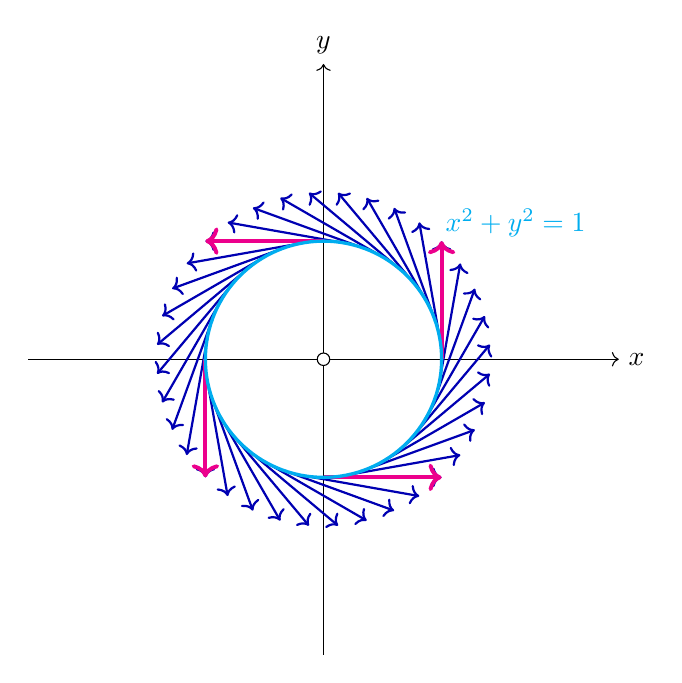
\begin{tikzpicture}[scale=1.5]
	%	\draw[dashed, gray!20] (-4,-4) grid (4,4);
	% Axes
	\draw[->] (-2.5,0) -- (2.5,0) node[right] {$x$};
	\draw[->] (0,-2.5) -- (0,2.5) node[above] {$y$};
	\fill[white,draw=black] (0,0) circle (1.5pt);
	\def\arrowlen{1}
	\foreach \t in {0,10,...,350}{
		\pgfmathsetmacro\x{cos(\t)}
		\pgfmathsetmacro\y{sin(\t)}
		% On r=1, F = (-y,x)
		\pgfmathsetmacro\dx{(-\y)*\arrowlen}
		\pgfmathsetmacro\dy{(\x)*\arrowlen}
		\draw[->, thick, blue!70!black] 
		(\x,\y) -- ++(\dx,\dy);
	}
	\foreach \t in {0,90,180,270}{
		\pgfmathsetmacro\x{cos(\t)}
		\pgfmathsetmacro\y{sin(\t)}
		% On r=1, F = (-y,x)
		\pgfmathsetmacro\dx{(-\y)*\arrowlen}
		\pgfmathsetmacro\dy{(\x)*\arrowlen}
		\draw[->, line width=.5mm, magenta] 
		(\x,\y) -- ++(\dx,\dy);
	}
	%--- Draw contour C with orientation --------------------
	\draw[cyan, very thick]
	(0,0) circle (1)
	node[above right=2cm] {$x^2+y^2=1$};
\end{tikzpicture}
\end{minipage}
\end{center}	
Consider the vector field:
\[
\vec{F}(x, y) = \left( \frac{-y}{x^2 + y^2},\; \frac{x}{x^2 + y^2} \right),
\]
and the curve \( C \) is the unit circle \( x^2 + y^2 = 1 \), traversed counterclockwise.

\begin{enumerate}[\bfseries Step 1.]
	\item \textbf{(Parametrization)} Define a function \[
	\fullfunction{\gamma}{[0,2\pi]}{\set{(x,y)\in\R^2:x^2+y^2=1}}{\theta}{\gamma(\theta)=(\cos\theta,\sin\theta)}.
	\] Here, $\frac{d\gamma}{d\theta}=(-\sin\theta,\cos\theta)$.
	\begin{center}
	\begin{minipage}{.4\textwidth}\centering
	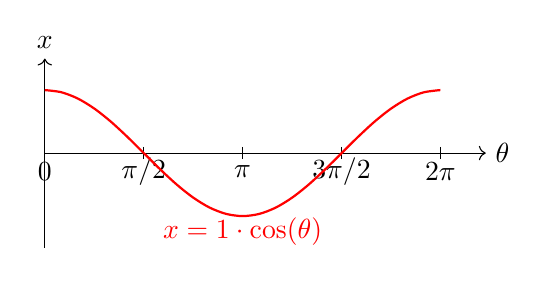
\begin{tikzpicture}[scale=.8]
		% Draw axes
		\draw[->] (0,-1.5) -- (0,1.5) node[above] {\(x\)};
		\draw[->] (0,0) -- (7,0) node[right] {\(\theta\)};
		
		% Mark key points on the t-axis (0, pi/2, pi, 3pi/2, 2pi)
		\foreach \x in {0,1.57,3.14,4.71,6.28} {
			\draw (\x,0.1) -- (\x,-0.1);
		}
		\node at (0,-0.3) {\(0\)};
		\node at (1.57,-0.3) {\(\pi/2\)};
		\node at (3.14,-0.3) {\(\pi\)};
		\node at (4.71,-0.3) {\(3\pi/2\)};
		\node at (6.28,-0.3) {\(2\pi\)};
		
		% Draw sin(t) in blue
	%	\draw[domain=0:6.28, smooth, variable=\t, blue, thick] 
	%	plot ({\t},{sin(\t r)});
	%	\node[blue] at (1.67,1.25) {\(\sin(t)\)};
		
		% Draw cos(t) in red
		\draw[domain=0:6.28, smooth, variable=\t, red, thick] 
		plot ({\t},{cos(\t r)});
		\node[red] at (3.14,-1.25) {\(x=1\cdot\cos(\theta)\)};
	\end{tikzpicture}
	\end{minipage}\hfill
	\begin{minipage}{.4\textwidth}\centering
	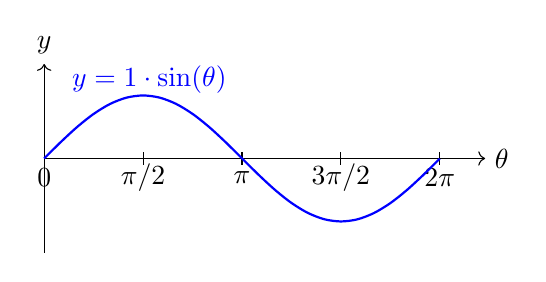
\begin{tikzpicture}[scale=.8]
		% Draw axes
		\draw[->] (0,-1.5) -- (0,1.5) node[above] {\(y\)};
		\draw[->] (0,0) -- (7,0) node[right] {\(\theta\)};
		
		% Mark key points on the t-axis (0, pi/2, pi, 3pi/2, 2pi)
		\foreach \x in {0,1.57,3.14,4.71,6.28} {
			\draw (\x,0.1) -- (\x,-0.1);
		}
		\node at (0,-0.3) {\(0\)};
		\node at (1.57,-0.3) {\(\pi/2\)};
		\node at (3.14,-0.3) {\(\pi\)};
		\node at (4.71,-0.3) {\(3\pi/2\)};
		\node at (6.28,-0.3) {\(2\pi\)};
		
		% Draw sin(t) in blue
		\draw[domain=0:6.28, smooth, variable=\t, blue, thick] 
		plot ({\t},{sin(\t r)});
		\node[blue] at (1.67,1.25) {\(y=1\cdot \sin(\theta)\)};
		
		% Draw cos(t) in red
	%	\draw[domain=0:6.28, smooth, variable=\t, red, thick] 
	%	plot ({\t},{cos(\t r)});
	%	\node[red] at (3.14,-1.25) {\(\cos(t)\)};
	\end{tikzpicture}
	\end{minipage}
	\end{center}
	\item \textbf{(Evaluate $\textbf{F}(\gamma(\theta))$ and the dot product)}\; We have \[
	\vec{F}(\gamma(\theta)) = \vec{F}(\cos\theta,\sin\theta) \overset{\sin^2\theta+\cos^2\theta=1}{=} \left( \frac{-\sin \theta}{1}, \frac{\cos \theta}{1} \right)
	= (-\sin \theta, \cos \theta).
	\] and \[
	\vec{F}(\gamma(\theta)) \cdot \frac{d\gamma}{d\theta}
	= (-\sin \theta)(-\sin \theta) + (\cos \theta)(\cos \theta)
	= \sin^2 \theta + \cos^2 \theta = 1.
	\]
	\item \textbf{(Integral)} \[
	\oint_C \vec{F} \cdot d\vec{r}
	= \int_0^{2\pi} \vec{F}(\gamma(\theta)) \cdot\frac{d\gamma}{d\theta}\,d\theta
	= \int_0^{2\pi} 1\,d\theta = 2\pi.
	\]
\end{enumerate}
\end{proof}


%\begin{thebibliography}{9}
%	\bibitem{riemann_0}
%	수학의 즐거움, Enjoying Math. ``[리만의 복소해석을 토대로 얻는 내 수학적 시야] 0. 오리엔테이션'' YouTube Video, 1:49:27. Published 
%	September 4, 2023. URL: \url{https://www.youtube.com/watch?v=EovxcF_DG_k&list=PL4m4z_pFWq2ob-P9m3SQZPyHTaJbbkvdz}.
%	\bibitem{riemann_1}
%	수학의 즐거움, Enjoying Math. ``[리만의 복소해석을 토대로 얻는 내 수학적 시야] 1. 선적분의 정의에 대한 디스커션'' YouTube Video, 1:58:19. Published 
%	September 11, 2023. URL: \url{https://www.youtube.com/watch?v=zoalSFi1RKo&list=PL4m4z_pFWq2ob-P9m3SQZPyHTaJbbkvdz&index=2}.
%\end{thebibliography}

%\newpage
%\appendix
%\section{Proof of Zorn's Lemma from Axiom of Choice}
%\thmbox{\begin{theorem*}\hypertarget{zorn}{}
%The following statements are equivalent: \begin{enumerate}
%	\item \textbf{Axiom of Choice (AC)}:\quad For every indexed family $\set{S_i}_{i\in I}$ of nonempty sets, there exists a choice function $f:I\to\bigcup_{i\in I}S_i$ such that $f(i)\in X_i$ for all $i\in I$.
%	\item \textbf{Zorn's Lemma}:\quad If $(P,\preceq)$ is a nonempty partially ordered set in which every chains has an upper bound in $P$, then $P$ contains at least one maximal element.
%\end{enumerate}
%\end{theorem*}}
%\begin{proof}
%\begin{itemize}
%	\item[($\Rightarrow$)] $(\textbf{AC}\implies \textbf{ZL})$ Assume that the Axiom of Choice holds.
%	\begin{enumerate}
%		\item \textbf{Definition of Poset}
%		
%		Let $(P,\preceq)$ be a nonempty partially ordered set with the property that every chain in $P$ has an upper bound in  $P$.
%		
%		\item \textbf{Construction of an Extending Function}
%		
%		Define the family $\set{\mathcal{C}_i}_{i\in I}$ of chains in $P$. For any chain $\mathcal{C}_i$ that is not maximal with respect to inclusion (\ie, $\exists $), AC guarantees that we can elect an element \[
%		f(C)
%		\] 
%	\end{enumerate}
%	\item[($\Leftarrow$)] $(\textbf{ZL}\implies \textbf{AC})$ 
%\end{itemize}
%\end{proof}

\newpage
\appendix
\section{Differential Geometry}

\end{document}
